\documentclass[conference]{IEEEtran}
\IEEEoverridecommandlockouts

\usepackage{cite}
\usepackage{amsmath,amssymb,amsfonts}
\usepackage{algorithmic}
\usepackage{graphicx}
\usepackage{textcomp}
\usepackage{xcolor}
\usepackage{booktabs}
\usepackage{array}
\usepackage{url}
\usepackage[hidelinks]{hyperref}

\graphicspath{{figures/}}

\begin{document}

\title{A Fine-Tuned Transformer for Criterion-Level\\ Clinical Trial Eligibility Screening with\\ Traceable Evidence and Efficient Inference}

\author{
\IEEEauthorblockN{Masooma Ali}
\IEEEauthorblockA{
% TODO: replace the three lines below with your real details before submission.
\textit{Department of Computer Science} \\
\textit{[Your University]} \\
Roll No. [XX-XXXX] \quad Course: Generative AI \\
masooma-ali@example.edu}
}

\maketitle

\begin{abstract}
Matching a patient to a clinical trial requires judging the patient record
against each inclusion and exclusion criterion individually and justifying
every decision with evidence from the record. We fine-tune an open-weight
decoder, Qwen2.5-1.5B-Instruct, with Low-Rank Adaptation (LoRA) on the TrialGPT
Criterion-Annotations dataset so that it reads a patient note, a criterion type,
and a criterion, and returns a structured eligibility label together with the
identifiers of the supporting patient sentences. All four expert categories per
criterion type are preserved, including \emph{not enough information} and
\emph{not applicable}, and any verdict that cites no sentence is flagged for
human review rather than treated as proof. Using a sealed, patient-grouped
37/8/8 split, fine-tuning raises held-out test macro-F1 from 0.234 (untrained
base) to 0.560 and accuracy from 0.204 to 0.728. Beyond accuracy, we implement
and validate three inference mechanisms from first principles against reference
paths under greedy decoding: an explicit key/value (KV) cache that reproduces
uncached tokens exactly while giving up to a 9.2$\times$ decode speed-up on long
inputs; a tiled online-softmax attention kernel that matches a reference
implementation to a maximum absolute error of $5\times10^{-7}$; and greedy
speculative decoding that produces token-identical output at a 90--97\% draft
acceptance rate, yet runs 15--24\% slower than plain greedy on our hardware---a
slowdown we measure and explain. The system is delivered as a browser
application that screens unseen notes, shows each verdict with its cited
evidence, and exposes a live benchmark of the decoding mechanisms. It is an
educational screening prototype, not a clinical enrollment tool.
\end{abstract}

\begin{IEEEkeywords}
clinical trial eligibility, clinical NLP, parameter-efficient fine-tuning, LoRA,
KV cache, FlashAttention, online softmax, speculative decoding, evidence
attribution.
\end{IEEEkeywords}

\section{Introduction and Problem Statement}
Recruiting patients into clinical trials is slow and expensive, largely because
screening a patient means reading a free-text record and checking it against a
long list of inclusion and exclusion criteria, each of which may be met, not
met, inapplicable, or impossible to decide from the available text. Large
language models can automate parts of this reasoning~\cite{jin2024trialgpt}, but
a system that merely emits ``eligible'' or ``ineligible'' is not trustworthy for
clinical use: a screening tool must say \emph{which} criterion drove a decision
and \emph{which} sentence of the record supports it, and it must distinguish
``the criterion is not satisfied'' from ``the record does not say.''

This work builds such a system under three constraints. First, it must run on
freely available hardware with open weights---no paid APIs or proprietary
models. Second, it must preserve the full label taxonomy of the benchmark and
attribute every decision to patient-record evidence. Third, beyond training a
classifier, it must demonstrate a genuine, verified understanding of modern
autoregressive inference: KV caching, efficient attention, and speculative
decoding, each implemented and checked against a reference rather than switched
on through a library flag.

\textbf{Contributions.} (1) A LoRA fine-tune of Qwen2.5-1.5B-Instruct for
criterion-level eligibility with evidence-sentence attribution, evaluated on a
sealed patient-grouped split with a documented before/after comparison. (2)
From-scratch implementations of a cache-aware greedy decoder, a tiled
online-softmax attention kernel, and greedy speculative decoding, each validated
for exact token or numerical agreement with a reference and benchmarked. (3) A
standalone browser application that performs criterion-level screening with
traceable evidence, aggregates a preliminary patient-level verdict by explicit
rules, and exposes a live inference-comparison view.

\section{Related Work}
\textbf{LLMs for trial matching.} TrialGPT~\cite{jin2024trialgpt} introduced the
criterion-level annotation task and a prompting pipeline over GPT-4; we reuse its
public annotations as the supervised benchmark but, as required, do not use its
model-generated predictions or explanations as inputs or labels. Our contribution
is a small, locally executable, \emph{fine-tuned} model with verified inference
internals rather than a closed-model prompting demonstration.

\textbf{Transformer architecture and attention.} The Transformer and scaled
dot-product attention~\cite{vaswani2017attention} underlie our target model.
FlashAttention~\cite{dao2022flashattention} shows that attention can be computed
tile-by-tile without materialising the full score matrix, using the online
softmax recurrence of Milakov and Gimelshein~\cite{milakov2018online}; our
educational kernel in Section~\ref{sec:attn} implements exactly this recurrence.

\textbf{Parameter-efficient adaptation.} LoRA~\cite{hu2022lora} freezes the base
weights and trains low-rank updates to selected projections, and
QLoRA~\cite{dettmers2023qlora} adds quantisation; with only 602 training rows,
full fine-tuning would overfit and exceed our memory budget, so we adopt LoRA.

\textbf{Speculative decoding.} Leviathan et
al.~\cite{leviathan2023speculative} and Chen et al.~\cite{chen2023accelerating}
accelerate decoding by drafting tokens with a small model and verifying them
with the target in one pass, guaranteeing the target's exact greedy output. We
implement the greedy variant and report where it does \emph{not} pay off.

\textbf{Model families.} We compare Qwen2.5~\cite{qwen2024report} and
SmolLM2~\cite{allal2025smollm2} as candidates and reject
Qwen3~\cite{qwen2025qwen3} for reasons given in Section~\ref{sec:model}.

\section{Materials and Methods}

\subsection{Dataset and Patient-Grouped Split}
We use only the TrialGPT Criterion-Annotations
dataset,\footnote{\url{https://huggingface.co/datasets/ncbi/TrialGPT-Criterion-Annotations}}
which contains 1{,}015 annotations over 53 patients: a patient description, a
single criterion with its type (inclusion/exclusion), an expert eligibility
label, and expert-identified evidence sentence IDs. To prevent leakage, we split
\emph{by patient}: unique patient IDs are sorted, shuffled with
\texttt{numpy.random.default\_rng(42)}, and assigned 37/8/8 to
train/validation/test. Every annotation for a patient stays in one split. One
row with a blank criterion (annotation 883) has nothing to judge and is removed
from training and scoring in all splits; the decision predates any results and
is recorded in the published manifest. Table~\ref{tab:split} summarises the
split, which yields 602 usable training rows, 206 validation, and 206 test. The
test split was sealed and read exactly once, for final evaluation.

\begin{table}[t]
\caption{Patient-grouped split (seed 42). The test split was not inspected
during development.}
\label{tab:split}
\centering
\begin{tabular}{lccc}
\toprule
Split & Patients & Rows (usable) & \\
\midrule
Train      & 37 & 602 & \\
Validation & 8  & 206 & \\
Test       & 8  & 206 & \\
\midrule
Total      & 53 & 1014 & (+1 removed) \\
\bottomrule
\end{tabular}
\end{table}

\subsection{Data Processing and Output Schema}
The loader requests only the eight columns it needs; the
\texttt{gpt4\_*} and \texttt{explanation\_correctness} columns are never read, so
prior model outputs cannot leak into inputs or labels. Each patient note is a
numbered list of sentences; we keep the original IDs so that predicted evidence
is traceable to the exact source sentence, and an NLTK splitter assigns IDs to
unseen notes in the application. The model is trained to emit a compact JSON
object, \texttt{\{"label": <category>, "evidence": [<ids>]\}}. The label space is
the dataset's own taxonomy: \{included, not included, not enough information, not
applicable\} for inclusion criteria and \{excluded, not excluded, not enough
information, not applicable\} for exclusion criteria. We deliberately keep
\emph{not enough information} and \emph{not applicable} as first-class outcomes
rather than collapsing to yes/no. Explanations are \emph{not} learned: the only
written explanations in the dataset are GPT-4's, which the rules bar; instead the
application states the verdict in fixed wording and quotes the cited sentences
verbatim, so an explanation cannot introduce an unsupported fact.

\textbf{Tokenisation and truncation.} Inputs use the Qwen2.5 chat template. The
application caps prompts at 2{,}048 tokens and \emph{refuses} longer inputs with
a message rather than silently truncating, because clipping a note could discard
the very sentence that constitutes the evidence. No training row exceeded the
limit, so no evidence was lost to truncation.

\subsection{Model Selection}
\label{sec:model}
We require an open-weight decoder that (i) fits a 4\,GB laptop GPU for the
application and a free 16\,GB Kaggle T4 for training, (ii) supports the
autoregressive inference work, and (iii) has a draft sibling with an identical
tokeniser for speculative decoding. Table~\ref{tab:models} lists the candidates.
We select \textbf{Qwen2.5-1.5B-Instruct} (Apache-2.0, 28 layers, 32k context) as
the target and \textbf{Qwen2.5-0.5B-Instruct} (24 layers) as the draft; the two
share an identical vocabulary of 151{,}665 tokens, special tokens and chat
template, which is a precondition for speculative verification.
SmolLM2-1.7B-Instruct is a reasonable alternative but did not fine-tune as well
(Section~\ref{sec:ft}). We reject the Qwen3 family: its ``thinking'' mode is on
by default and injects reasoning text that complicates structured JSON output,
and the 4B variant needs $\approx$8\,GB at float16, exceeding the laptop GPU.

\begin{table}[t]
\caption{Open-weight decoder candidates. All Apache-2.0.}
\label{tab:models}
\centering
\begin{tabular}{lccc}
\toprule
Model & Params & Layers & Role \\
\midrule
Qwen2.5-1.5B-Instruct & 1543.7M & 28 & \textbf{target (chosen)} \\
Qwen2.5-0.5B-Instruct & 494.0M  & 24 & \textbf{draft (chosen)} \\
SmolLM2-1.7B-Instruct & 1711.4M & 24 & candidate, rejected \\
\bottomrule
\end{tabular}
\end{table}

\subsection{Fine-Tuning with LoRA}
\label{sec:ft}
We adapt the target with LoRA~\cite{hu2022lora} on the attention projections
(\texttt{q,k,v,o\_proj}) at rank 32, $\alpha{=}64$, dropout 0.05, training
8.72M parameters---0.56\% of the 1.55B total. Optimisation uses AdamW,
learning rate $2{\times}10^{-4}$, batch size 4 with 2 gradient-accumulation
steps, 10\% warmup, gradient clipping at 1.0, and gradient checkpointing. The
objective is standard next-token cross-entropy over the JSON target. Decoding for
all evaluation is \emph{greedy} with repetition penalty fixed to 1.0; Qwen's
bundled generation config enables sampling, which we override explicitly so that
before/after comparisons are deterministic and token-equality with our custom
decoders holds. Because the mandatory split leaves only 8 ``excluded'' and 13
``not included'' training rows, we optionally oversample rare labels in training
by a power of 0.5. All hyperparameters and the final checkpoint were chosen on
validation data only; early stopping used patience 2 on validation macro-F1.
Training the selected configuration took $\approx$1{,}295\,s on a T4 at a 7.55\,GB
peak.

\subsection{KV-Cached Autoregressive Decoding}
\label{sec:kv}
Autoregressive generation recomputes attention over all previous tokens at every
step. We implement an explicit cache-aware decoder that, after a prefill pass
over the prompt, stores each layer's key and value tensors and, for every new
token, runs a \emph{single-token} forward pass that appends one key/value row per
layer and attends over the stored cache. Correct positional handling is
essential: the new token's rotary position index is the running cache length, not
0. The causal mask is implicit, because a one-row query can only attend to keys
that already exist. We also build an \emph{uncached} reference decoder that
reprocesses the whole growing sequence each step, giving an independent oracle
for token-equality tests. Minor numerical differences between the two paths are
expected and bounded (Section~\ref{sec:kvres}) because the cached path changes
the reduction order of floating-point attention.

\subsection{Tiled Online-Softmax Attention}
\label{sec:attn}
We implement reference scaled dot-product attention---$\mathrm{softmax}(QK^\top/
\sqrt{d_k}\,{+}\,M)V$ with a numerically stable max-subtraction---and a tiled
variant following FlashAttention~\cite{dao2022flashattention}. The tiled kernel
walks key/value blocks while maintaining, per query, a running maximum $m$, a
running normaliser $\ell$, and a running weighted sum, rescaling previous
contributions by $e^{m_{\text{old}}-m_{\text{new}}}$ as the maximum
grows~\cite{milakov2018online}; it never materialises the full $N{\times}N$ score
matrix. Under a causal mask, blocks that lie entirely in the future are skipped.
Both are tested on small controlled inputs for agreement
(Section~\ref{sec:attnres}).

\subsection{Speculative Decoding}
\label{sec:spec}
Our greedy speculative decoder drafts $k$ tokens with the 0.5B model, then runs
\emph{one} target forward pass over the drafted block to obtain the target's
greedy token at each position. It accepts the longest prefix on which draft and
target agree, always appends the target's own next token (so at least one token
is committed per round even under full rejection), and rolls both models' KV
caches back to the accepted length to keep state consistent. Because every
committed token is the target's greedy choice, the output is provably identical
to plain greedy target decoding, which we verify in Section~\ref{sec:specres}.

\subsection{Application Workflow}
The system is a FastAPI server that loads the model once and serves a React/Vite
single-page interface (Fig.~\ref{fig:app}). A user pastes or uploads a note,
reviews the auto-numbered sentences, enters or imports inclusion/exclusion
criteria, and runs the screening; a single-GPU job queue processes one request at
a time. Each criterion returns its predicted category, cited sentence IDs,
extracted evidence text, and a fixed-wording explanation. A patient-level verdict
is produced only as an explicit rule-based \emph{aggregation}
(``likely ineligible'' if any criterion fails with cited evidence; otherwise
``needs review'' if anything is unknown, unverified, or uncited; otherwise
``potentially eligible''), labelled preliminary, and never presented as a
separately ground-truthed outcome. The interface exposes a live benchmark view
(Fig.~\ref{fig:appbench}) that runs the three decoders and the two attention
kernels on demand, and exports a self-contained HTML/JSON report carrying the
model and adapter provenance. A banner states that the tool is an educational
prototype.

\begin{figure}[t]
\centering
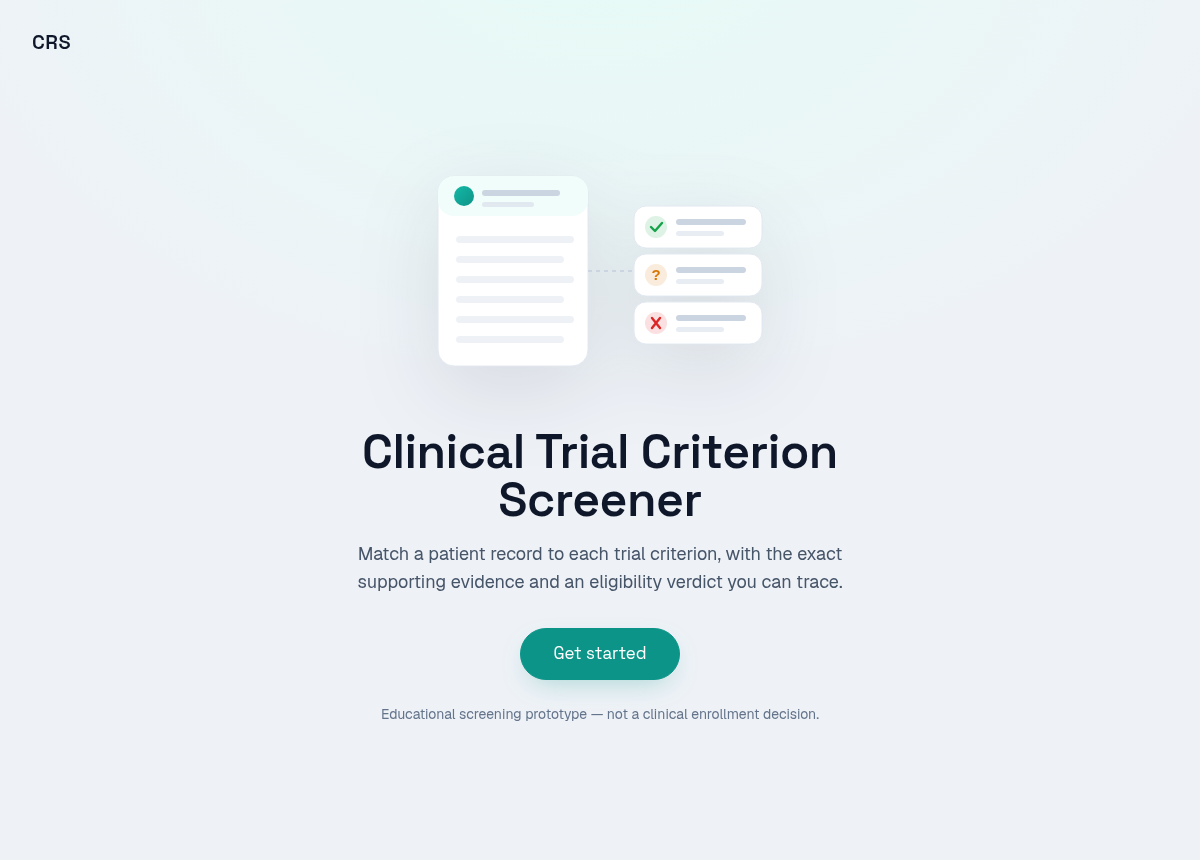
\includegraphics[width=0.92\columnwidth]{app_landing.png}
\caption{Browser application: a patient record is matched to each trial
criterion with traceable evidence. The prototype notice is shown throughout.}
\label{fig:app}
\end{figure}

\section{Experimental Setup and Metrics}
\textbf{Hardware.} Fine-tuning and full benchmarks ran on a free Kaggle Tesla T4
(16\,GB). The application, tests, and small benchmarks ran on a laptop
(i7-11800H, RTX 3050 Ti 4\,GB); the deployment target in this report is a
CPU-only machine on which the application also runs (slower, float32).

\textbf{Metrics.} For classification we report accuracy and macro-F1, per-class
precision/recall/F1, and confusion matrices, overall and separately for inclusion
vs.\ exclusion. For evidence retrieval we report sentence-level micro and macro
precision/recall/F1; rows where both gold and predicted evidence are empty count
as perfect (F1\,=\,1), and the fraction of such rows is reported so the macro
number is not misread. For inference we report prefill time, decode time,
tokens/s, peak memory, draft acceptance rate, and token-equality against the
reference, with warm-up discarded and medians over repeated runs.

\section{Results and Discussion}

\subsection{Fine-Tuning and Before/After}
\label{sec:ftres}
Table~\ref{tab:runs} compares all runs on validation data. The untrained base
(R0) scores 0.147 macro-F1; LoRA fine-tuning (R1--R4) more than triples this.
Oversampling rare labels helps (R2 over R1), and rank 32 with oversampling (R3)
gives the best validation macro-F1 (0.558) and the best evidence F1 among the
Qwen runs, so \textbf{R3 is selected by the pre-stated rule}. Putting evidence
before the label (R4) slightly raised evidence F1 but hurt label macro-F1 to
0.459, so the label-first format was kept. SmolLM2 (R5) and the 0.5B draft (R6)
trained but scored lower, confirming the target choice.
Fig.~\ref{fig:train} shows R3's training: training loss falls monotonically while
validation loss and macro-F1 diverge after epoch~4, which the patience-2 rule
correctly selects as the checkpoint.

\begin{table}[t]
\caption{Validation results across runs. \texttt{os}: oversample power,
\texttt{rk}: LoRA rank. R3 (bold) is selected. All macro-F1 over the six scored
labels.}
\label{tab:runs}
\centering
\small
\begin{tabular}{llccccc}
\toprule
Run & Model & rk & os & Acc. & Macro-F1 & Ev-F1 \\
\midrule
R0  & Qwen-1.5B (base) & 16 & -- & 0.175 & 0.147 & 0.106 \\
R0b & SmolLM2 (base)   & 16 & -- & 0.180 & 0.120 & 0.111 \\
R1  & Qwen-1.5B        & 16 & 0   & 0.752 & 0.534 & 0.462 \\
R2  & Qwen-1.5B        & 16 & 0.5 & 0.738 & 0.552 & 0.487 \\
\textbf{R3} & \textbf{Qwen-1.5B} & \textbf{32} & \textbf{0.5} & \textbf{0.743} & \textbf{0.558} & \textbf{0.509} \\
R4  & Qwen-1.5B (ev-first) & 32 & 0.5 & 0.762 & 0.459 & 0.526 \\
R5  & SmolLM2          & 32 & 0.5 & 0.675 & 0.514 & 0.446 \\
R6  & Qwen-0.5B (draft)& 32 & 0.5 & 0.738 & 0.446 & 0.491 \\
\bottomrule
\end{tabular}
\end{table}

\begin{figure}[t]
\centering
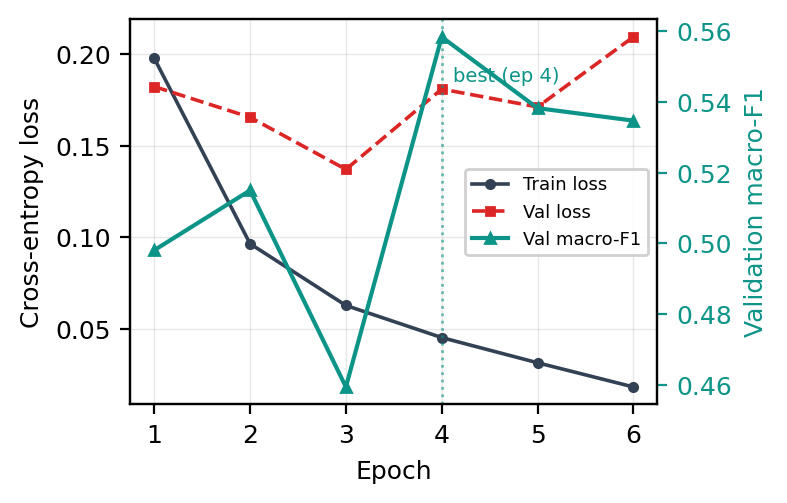
\includegraphics[width=0.95\columnwidth]{training_curves.png}
\caption{Run R3 training. Validation loss and macro-F1 diverge after epoch~4
(dotted), the selected checkpoint.}
\label{fig:train}
\end{figure}

On the \textbf{sealed test split}, fine-tuning raises accuracy from 0.204 to
0.728 and macro-F1 from 0.234 to 0.560 (Table~\ref{tab:beforeafter}). A
majority-label baseline reaches 0.626 accuracy but only 0.272 macro-F1,
confirming that the accuracy gain is not merely from predicting the most common
class. Validation and test numbers agree closely (0.558 vs.\ 0.560 macro-F1),
indicating the configuration did not overfit the validation split.

\begin{table}[t]
\caption{Before/after on identical held-out examples, greedy decoding.}
\label{tab:beforeafter}
\centering
\begin{tabular}{llcc}
\toprule
Split & System & Accuracy & Macro-F1 \\
\midrule
Validation & Base (untrained) & 0.175 & 0.147 \\
Validation & LoRA (R3)        & 0.743 & 0.558 \\
\midrule
Test & Base (untrained)       & 0.204 & 0.234 \\
Test & Majority-label         & 0.626 & 0.272 \\
Test & \textbf{LoRA (R3)}     & \textbf{0.728} & \textbf{0.560} \\
\bottomrule
\end{tabular}
\end{table}

\subsection{Criterion Classification}
Table~\ref{tab:perclass} gives per-class test results. The model is strong on the
common verdicts---\emph{included} (F1 0.826, precision 1.0) and \emph{not
excluded} (F1 0.829)---and on \emph{not enough information} (F1 0.635). It is weak
on the rare and subtle classes: \emph{not applicable} (F1 0.286) and \emph{not
included} (F1 0.222, recall 1/7). The \emph{excluded} class has no test examples,
so its performance is unmeasurable on this split. Split by criterion type,
inclusion accuracy is 0.773 (macro-F1 0.469) and exclusion accuracy 0.702
(macro-F1 0.427); the confusion matrix (Fig.~\ref{fig:conf}) shows the dominant
error is predicting \emph{not excluded} / \emph{not enough information} where the
gold is a rarer decisive label.

\begin{table}[t]
\caption{Per-class results on the test split (R3). ``--'': no support.}
\label{tab:perclass}
\centering
\small
\begin{tabular}{lcccc}
\toprule
Class & Prec. & Recall & F1 & Support \\
\midrule
included              & 1.000 & 0.704 & 0.826 & 27 \\
not included          & 0.500 & 0.143 & 0.222 & 7 \\
not excluded          & 0.731 & 0.956 & 0.829 & 91 \\
not enough information& 0.667 & 0.606 & 0.635 & 66 \\
not applicable        & 0.500 & 0.200 & 0.286 & 15 \\
excluded              & -- & -- & -- & 0 \\
\bottomrule
\end{tabular}
\end{table}

\begin{figure}[t]
\centering
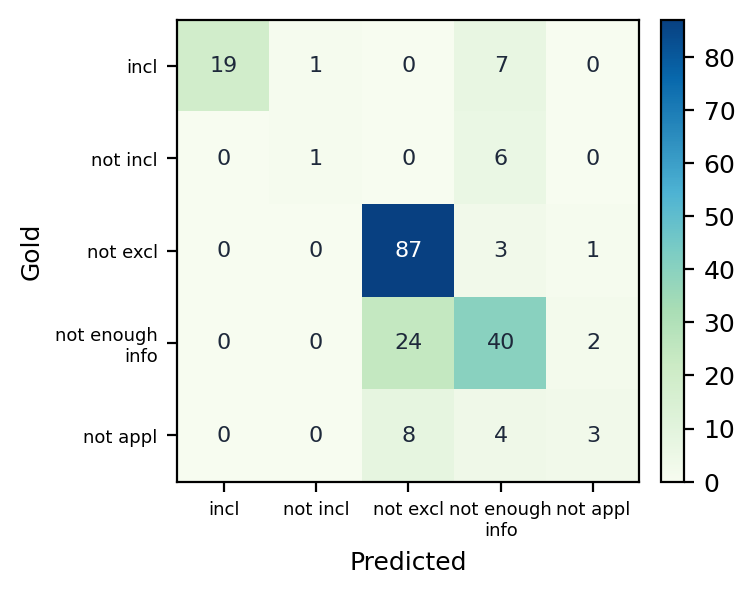
\includegraphics[width=0.82\columnwidth]{confusion_test.png}
\caption{Test confusion matrix (R3). Errors concentrate in the ``not enough
information'' and ``not excluded'' columns.}
\label{fig:conf}
\end{figure}

\subsection{Evidence Retrieval}
Sentence-level evidence retrieval on the test split reaches micro-F1 0.523
(precision 0.577, recall 0.479). Of 206 rows, 136 have both gold and predicted
evidence empty, 37 have both non-empty, 24 have gold evidence the model missed,
and 9 have evidence the model added where the gold had none. Restricted to the 61
rows with gold evidence, macro-F1 is 0.528; for inclusion criteria specifically,
evidence micro-F1 is 0.631. The large empty/empty count reflects that many
``not excluded'' verdicts are reached because a condition is simply never
mentioned---which is precisely why the application never reads an empty citation
as proof.

\subsection{Error Analysis}
A manual review of the 56 misclassified test rows (and 27 label-correct rows with
different evidence) identifies two systematic habits. On \emph{exclusion}
criteria the model defaults to \emph{not excluded}: 32 of 56 errors, learned from
training data in which 74.7\% of ``not excluded'' rows carry no cited sentence.
On \emph{inclusion} criteria it retreats to \emph{not enough information} when a
clinical inference is needed, giving that class recall 1.0 but ``not included''
recall 0.14. A representative failure is a negated inclusion criterion---``no
history of central venous catheterization''---where the note mentions arterial
catheterization; the shared word triggers a polarity flip. Crucially, because
that verdict cites no sentence, the application flags it and routes the patient to
``needs review'' rather than asserting ineligibility, so the user-facing failure
mode is caution, not a false decision. The largest error cluster (17 rows) comes
from one patient on one long trial, and the patient-level bootstrap interval for
macro-F1 is wide (0.43--0.64) given only 8 test patients---results should be read
with that uncertainty.

\subsection{KV Cache Benchmark}
\label{sec:kvres}
Across input lengths of 64--1024 and output lengths of 16--256, the cached
decoder produced \emph{token-identical} output to the uncached reference at every
setting, with a maximum absolute logit difference of 0.055 (mean 0.006), as
expected from reordered floating-point reductions. Fig.~\ref{fig:kv} shows decode
throughput: the uncached path slows sharply as the input grows (its per-step cost
scales with sequence length), while the cached path holds $\approx$25.5 tokens/s.
The speed-up therefore grows with input length, from 1.1$\times$ at 64 tokens to
8.4$\times$ at 1024 tokens (9.2$\times$ at 256 output tokens). This is the central
practical benefit of KV caching and is exactly what the clinical setting needs,
where prompts (note + criterion) are long.

\begin{figure}[t]
\centering
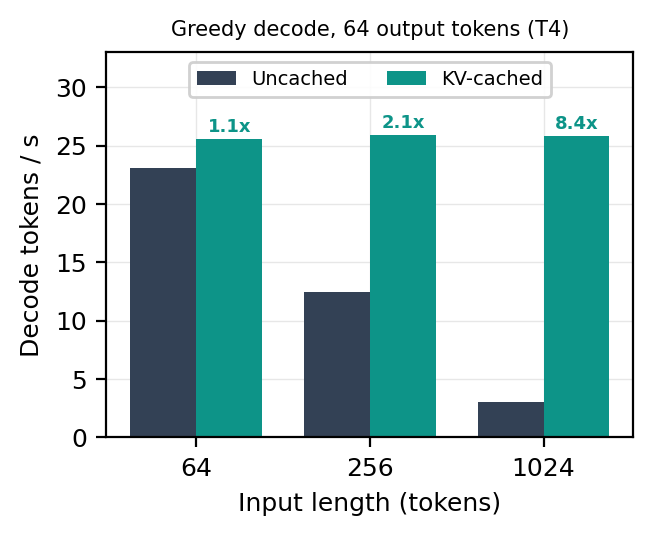
\includegraphics[width=0.95\columnwidth]{kv_cache.png}
\caption{KV-cache decode throughput on a T4. Labels show cached/uncached
speed-up; output identical to the reference at every point.}
\label{fig:kv}
\end{figure}

\subsection{Attention Benchmark}
\label{sec:attnres}
On controlled inputs with a causal mask, the tiled online-softmax kernel matched
the reference to a maximum absolute error of $5\times10^{-7}$ (mean
$2.6\times10^{-8}$), confirming correctness, and correctly skipped future blocks
(e.g.\ 6 of 16 tiles skipped at length 64, tile 16). On runtime
(Fig.~\ref{fig:attn}), however, the educational tiled kernel is \emph{slower}
than both the naive reference and PyTorch's fused backend---at length 4096 it
takes several milliseconds versus a fraction of a millisecond for the fused path.
This is expected: our kernel is pure Python/PyTorch and launches many small
operations per tile, whereas FlashAttention's advantage~\cite{dao2022flashattention}
comes from a single fused CUDA kernel that keeps tiles in on-chip SRAM. The
exercise demonstrates the algorithm's memory behaviour (no full score matrix),
not a faster kernel.

\begin{figure}[t]
\centering
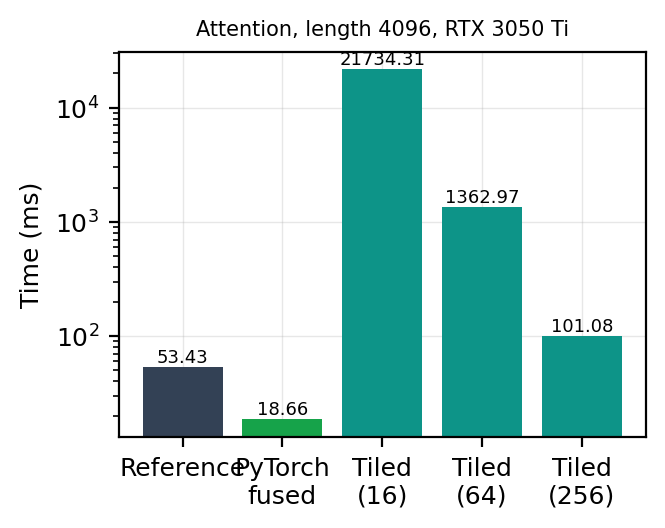
\includegraphics[width=0.9\columnwidth]{attention.png}
\caption{Attention runtime (log scale), length 4096. The educational tiled kernel
is correct but slower than the fused backend.}
\label{fig:attn}
\end{figure}

\subsection{Speculative Decoding Benchmark}
\label{sec:specres}
With the fine-tuned 0.5B draft, speculative decoding produced output identical to
greedy target decoding at every draft length $k\in\{2,4,8\}$, verifying
correctness. Draft acceptance was high---0.97 at $k{=}2$, 0.90 at $k{=}8$---yet
end-to-end throughput was \emph{lower} than plain greedy: 0.76$\times$ at $k{=}2$
to 0.85$\times$ at $k{=}8$ (Table~\ref{tab:spec}). The reason is the cost model:
the target's single-token decode is already cheap on a T4, so the extra draft
forward passes and the per-round verification overhead outweigh the tokens saved,
especially on the short structured outputs this task produces. Speculative
decoding pays off when the target step is expensive relative to the draft and
outputs are long; neither holds strongly here. As the rubric anticipates, we
report this slowdown honestly---the implementation is correct and the cache state
is maintained; it simply does not accelerate this workload.

\begin{table}[t]
\caption{Greedy speculative decoding vs.\ greedy target (T4, fine-tuned draft,
20 prompts). Output token-identical to greedy in all cases.}
\label{tab:spec}
\centering
\begin{tabular}{lccc}
\toprule
Mode & Tokens/s & Acceptance & Speed-up \\
\midrule
Greedy target     & 23.9 & --   & 1.00$\times$ \\
Speculative $k{=}2$ & 18.2 & 0.97 & 0.76$\times$ \\
Speculative $k{=}4$ & 19.3 & 0.91 & 0.81$\times$ \\
Speculative $k{=}8$ & 20.2 & 0.90 & 0.85$\times$ \\
\bottomrule
\end{tabular}
\end{table}

\begin{figure}[t]
\centering
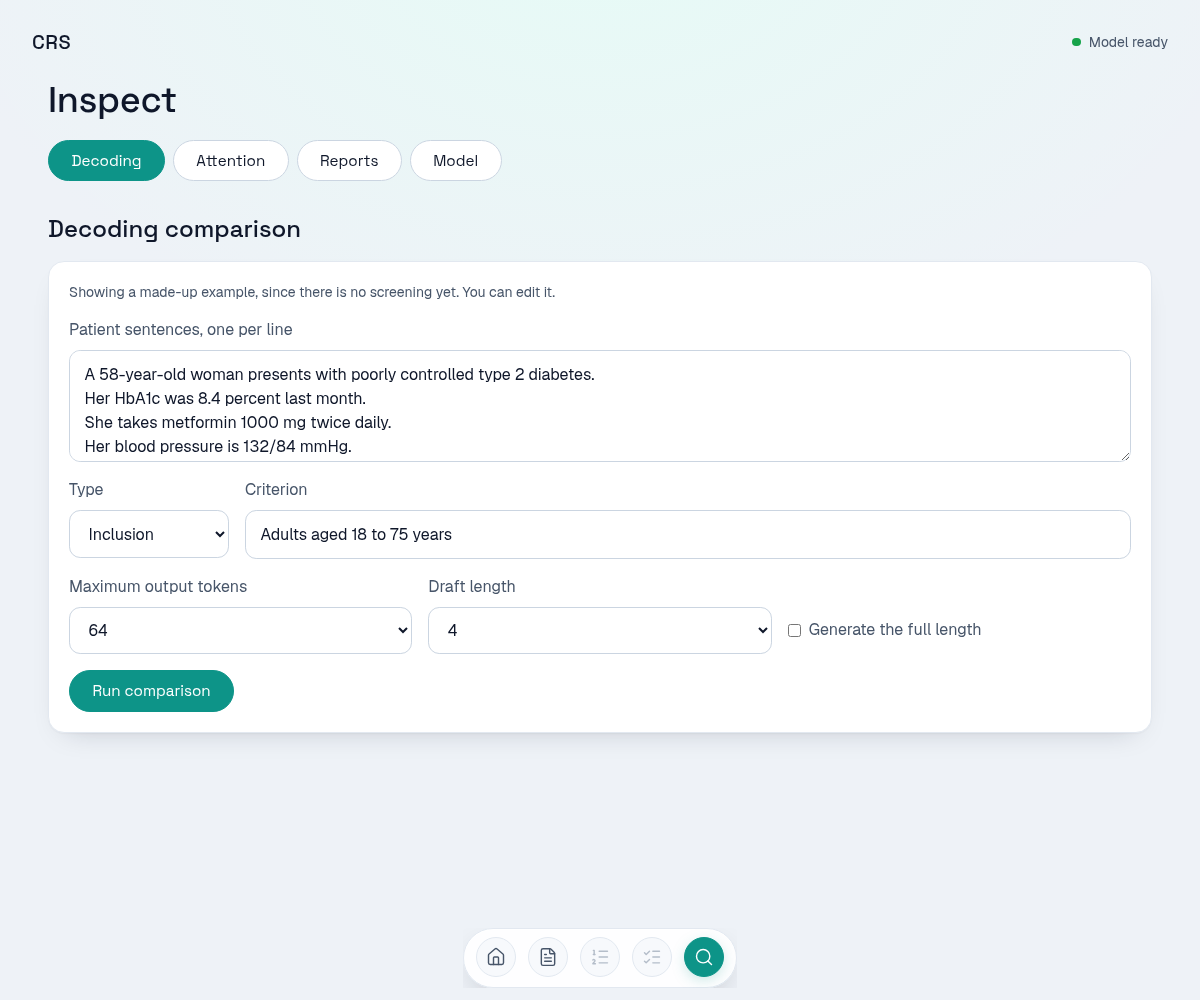
\includegraphics[width=0.95\columnwidth]{app_benchmark.png}
\caption{In-application benchmark view: the three decoders run on demand and are
compared on throughput, memory and token-equality.}
\label{fig:appbench}
\end{figure}

\section{Limitations}
The mandatory split gives only 8 test patients, so metrics carry wide
patient-level intervals and the \emph{excluded} class cannot be measured at all.
The model inherits the dataset's bias toward ``not excluded''/``not enough
information'' and is weak on rare decisive labels. Evidence recall (0.48) means
roughly half of gold citations are missed, though the application's
flag-for-review behaviour mitigates the risk of over-confident decisions. Our
attention and speculative implementations are educational: correct but not
faster than optimised backends on this hardware. Finally, the system is a
research screening prototype; it must not be used for real enrollment decisions.

\section{Conclusion}
We presented a locally executable, LoRA-fine-tuned Transformer that screens
patients against individual trial criteria, preserves the full expert label
taxonomy, and attributes every verdict to patient-record sentences, lifting
held-out macro-F1 from 0.234 to 0.560. We implemented and verified three
inference mechanisms from first principles: a KV cache that is token-exact and up
to 9.2$\times$ faster on long inputs, a tiled online-softmax attention kernel
matching a reference to $5\times10^{-7}$, and greedy speculative decoding that is
token-identical at 90--97\% acceptance but slower on this workload---a result we
measure and explain. The whole system is delivered as a browser application with
traceable evidence and a live inference benchmark. Future work includes
calibrated abstention on rare labels, better evidence recall, and evaluation on
additional patient cohorts.

\bibliographystyle{IEEEtran}
\bibliography{references}

\end{document}
